\chapter{Perceptual Image Compression}

Prakash2017 \cite{Prakash2017} introduced a powerful CNN
tailored to the specific task of semantic image understanding to achieve higher visual quality in lossy compression. A modest increase in complexity is incorporated into the encoder which allows a standard, off-the-shelf jpeg decoder to be used. While JPEG encoding may be optimized for generic images, the process is ultimately unaware of the specific content of the image to be compressed. This technique makes JPEG content-aware by designing and training a model to identify multiple semantic regions in a given image.


\section{Content aware compression}

The existing compression standards are content unware. For example, consider the case of JPEG algorithm, during the quantization step the quantization tables that are used are experimentally decided on a well-established theory that humans are insensitive to chrominance in contrast to luminance. An obvious question is can't we have a quantization table tailored specifically for each image. Of course, determining this table manually is a very uncertain and difficult task, and its well suited for the machine to do this for us.

The idea here is to locate multiple regions of interest (ROI) within a single image and noting the fact that it's not an object detection problem and hence the precision of the boundary doesn't matter. Also, the model needs to learn a single class-invariant feature map by learning separate feature maps for each of a set of object classes and then summing over the top features.

\section{Object Localization using CNNs}

\begin{figure}[!ht]
    \centering
    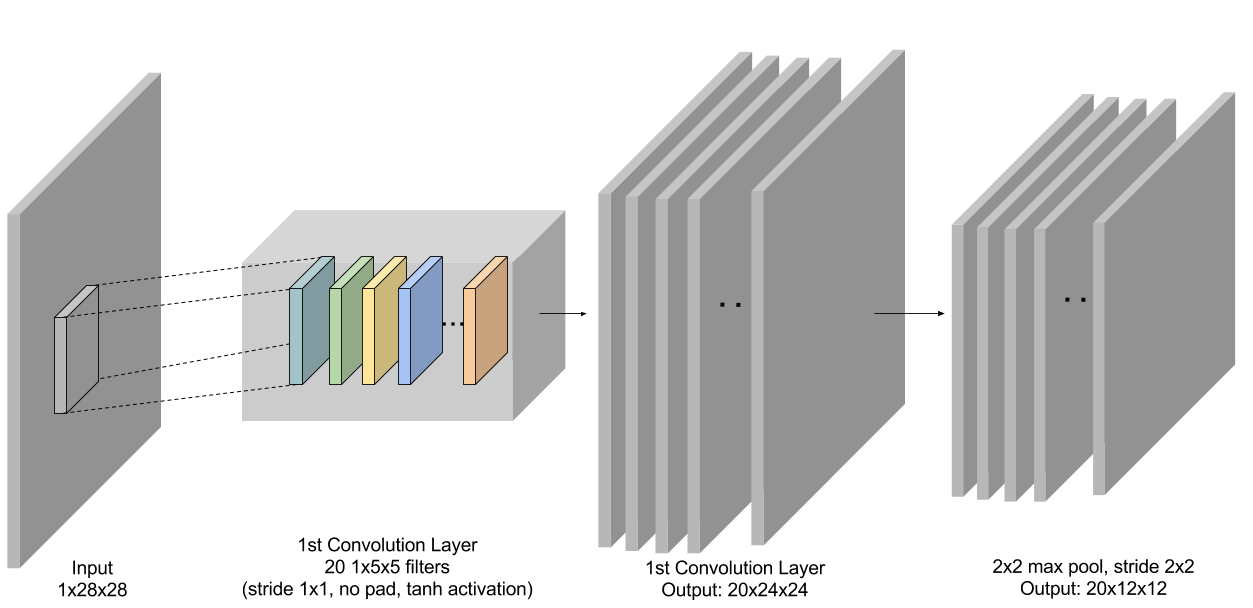
\includegraphics[width=0.65\textwidth]{fig/4-1.png}
    \captionsource{First convolutional layer in LeNet}
    {\href{https://mxnet.apache.org/api/python/docs/tutorials/packages/gluon/image/mnist.html}{https://mxnet.apache.org/}}
    \label{fig:firstConvLayerLeNet}
\end{figure}

CNNs are multi-layered feed-forward architectures where the learned features at each level are the weights of the convolution filters to be applied to the output of the previous level. Learning is done via gradient-based optimization. CNNs differ from FCNNs in that the dimensions of the learned convolution filters are, in general, much smaller than the dimensions of the input image, so the learned features are forced to be localized in space. Also, the convolution operation uses the same weight kernel at every image location, so feature detection is spatially invariant.

CNNs include a max-pooling step after every or every other layer of convolution, in which the height and width of the feature map (filter response) are reduced by replacing several neighboring activations (coefficients), generally within a square window, with a single activation equal to the maximum within that window. 

This pooling operation is strided, but the size of the pooling window can be greater than the stride, so windows can overlap. This results in down-sampling of input data, and filters applied to such a map will have a larger receptive field (spatial support in the pixel space) for a given kernel size, thus reducing the number of parameters of the CNN model and allowing the training of much deeper
networks. This does not change the depth of the feature map, but only its width and height. In practice, pooling windows are generally of size $2 \times 2$ or $4 \times 4$, with a stride of two, which reduces the number activations by $75 \%$.

Region-based CNNs use a moving window to maximize the posterior of the presence of an object. Recently many approaches have been proposed for object localization but either they are computationally expensive or they are limited to determine the presence/absence of a single class of object within an image. Moving-window methods can localize multiple objects but can't produce object silhouettes. In contrast, recent deep learning models proposed for semantic segmentation can produce a close object boundary but do not scale well for more than a small number of object categories. The proposed method only requires a rough idea but clear enough image-object map.

\vspace{2em}

\begin{figure}[!ht]
    \centering
    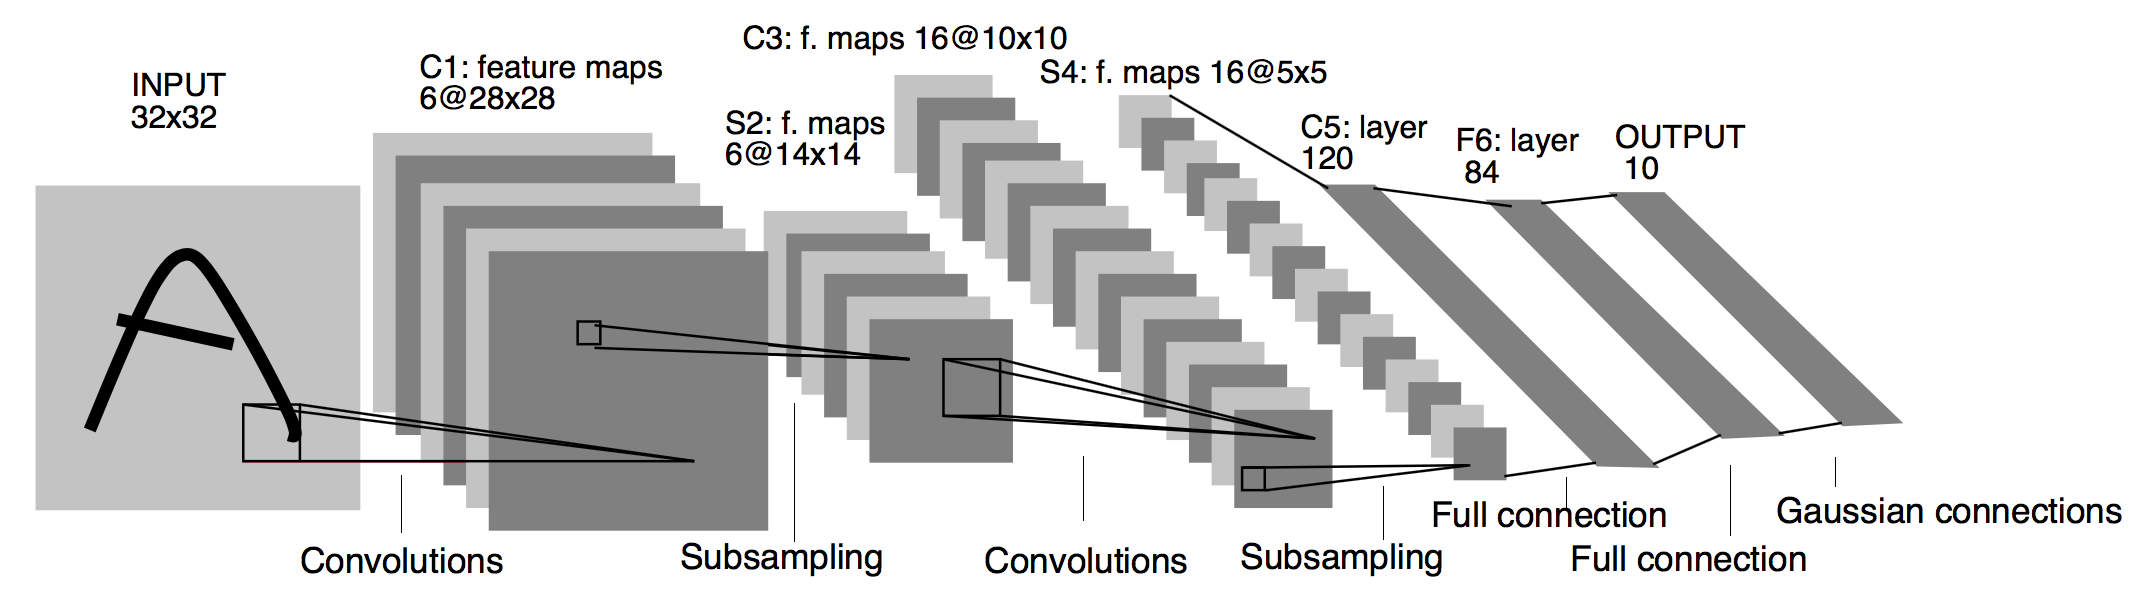
\includegraphics[width=0.80\textwidth]{fig/4-2.png}
    \captionsource{LeNet : a traditional CNN}
    {\href{https://medium.com/@pechyonkin/key-deep-learning-architectures-lenet-5-6fc3c59e6f4}{medium.com/@pechyonkin/}}
    \label{fig:LeNet}
\end{figure}

Unlike traditional CNNs where the last two layers are fully-connected, the authors of \cite{Oquab2015} and \cite{Zhou2016} modified the second to last layer to allow for class localization.

\begin{figure}[!ht]
    \centering
    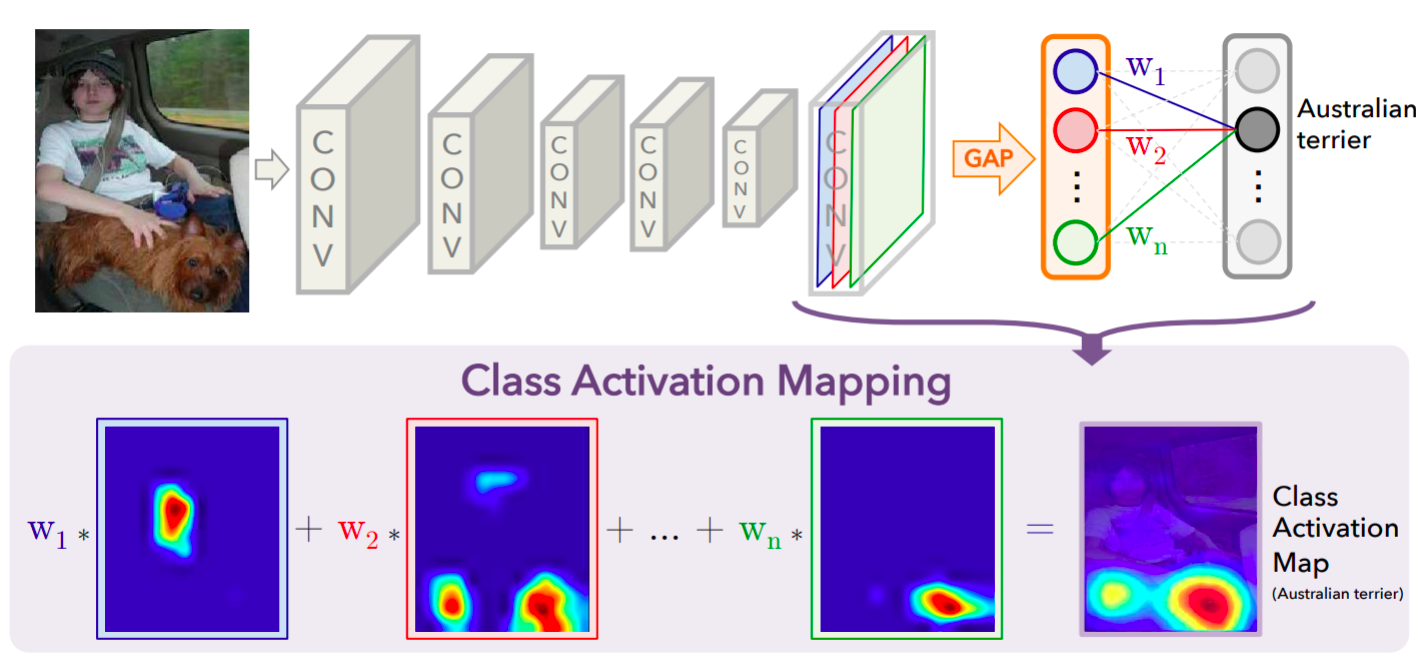
\includegraphics[width=0.80\textwidth]{fig/4-3.png}
    \captionsource{Class Activation Mapping: the predicted class score is mapped back to the previous convolutional layer to generate the class activation maps (CAMs). The CAM highlights the class-specific discriminative regions.}
    {Zhou2016 \cite{Zhou2016}}
    \label{fig:LeNet}
\end{figure}

\section{Multi-Structure Region of Interest}



\section{MS-ROI and JPEG}


\section{Model}

\section{Conclusion}
In this chapter, we proposed another distributed algorithm for
XYZ. This algorithm has both time complexity of $O(n)$ where $n$
is the total number of nodes.  In next chapter, we conclude and
discuss some of the future aspects.

